\section{Trabalhos Relacionados}
  \begin{frame}[fragile]{Matrizes de Referência}
    Silva (2017) explica em seu estudo, a prova de redação do ENEM é avaliada levando em conta uma matriz de referência elaborada pelo INEP ~\cite{silvio_taynan:2017}.
    \begin{table}[H]
    \fontsize{8}{10}\selectfont
    \centering
    % \caption{My caption}
    \label{table:matriz_referencia}
    \begin{tabular}{c|l|c|}
    \cline{2-3}
                                       & \multicolumn{1}{c|}{\textbf{Descrição}}                                                                                                                                                                                                       & \textbf{Valor} \\ \hline
    \multicolumn{1}{|c|}{\textbf{I  }} & \begin{tabular}[c]{@{}l@{} p{2cm}}Demonstrar domínio da norma padrão da língua escrita.\end{tabular}                                                                                                                                                 & \textit{200}            \\ \hline
    \multicolumn{1}{|c|}{\textbf{II }} & \begin{tabular}[c]{@{}l@{} p{2cm}}Compreender a proposta de redação e aplicar conceitos \\ das,varias áreas de conhecimento para desenvolver o \\ tema, dentro,dos limites estruturais do texto \\ dissertativo-argumentativo em,prosa.\end{tabular} & \textit{200}            \\ \hline
    \multicolumn{1}{|c|}{\textbf{III}} & \begin{tabular}[c]{@{}l@{} p{2cm}}Selecionar, relacionar, organizar e interpretar informações, \\ fatos, opiniões e argumentos em defesa de um ponto de \\vista.\end{tabular}                                                                        & \textit{200}            \\ \hline
    \multicolumn{1}{|c|}{\textbf{IV }} & \begin{tabular}[c]{@{}l@{} p{2cm}}Demonstrar conhecimento dos mecanismos linguísticos, \\ necessários para a construção da argumentação.\end{tabular}                                                                                                & \textit{200}            \\ \hline
    \multicolumn{1}{|c|}{\textbf{V  }} & \begin{tabular}[c]{@{}l@{} p{2cm}}Elaborar proposta de intervenção para o problema \\abordado, respeitando os direitos humanos.\end{tabular}                                                                                                         & \textit{200}            \\ \hline
    \end{tabular}
    \end{table}
  \end{frame}

  \begin{frame}[fragile]{Matrizes de Referência}
    \begin{table}[H]
    \fontsize{8}{10}\selectfont
    \centering
    % \caption{My caption}
    \label{table:competencia_iii}
    \begin{tabular}{|c|l|c|}
    \hline
    \multicolumn{3}{|l|}{\begin{tabular}[c]{@{}l@{}}\textbf{III} -- Selecionar, relacionar, organizar e interpretar informações, fatos, \\ opiniões e argumentos em defesa de um ponto de vista.\end{tabular}}                                                  \\ \hline
    \textbf{Nível} & \multicolumn{1}{c|}{\textbf{Descrição}}                                                                                                                                                                          & \textbf{Valor} \\ \hline
    \textbf{1}     & \begin{tabular}[c]{@{}l@{}}Apresenta informações, fatos e opiniões relacionados ao \\ tema proposto, de forma consistente e organizada, \\ configurando autoria, em defesa de um ponto de vista.\end{tabular}    & \textit{200}   \\ \hline
    \textbf{2}     & \begin{tabular}[c]{@{}l@{}}Apresenta informações, fatos e opiniões relacionados ao \\ tema, de forma organizada, com indícios de autoria, em \\ defesa de um ponto de vista.\end{tabular}                        & \textit{150}   \\ \hline
    \textbf{3}     & \begin{tabular}[c]{@{}l@{}}Apresenta informações, fatos e opiniões relacionados ao \\ tema, limitados aos argumentos dos textos motivadores \\ e pouco organizados, em defesa de um ponto de vista.\end{tabular} & \textit{100}   \\ \hline
    \textbf{4}     & \begin{tabular}[c]{@{}l@{}}Apresenta informações, fatos e opiniões pouco \\ relacionados ao tema ou incoerentes e sem defesa de um \\ ponto de vista.\end{tabular}                                               & \textit{50}    \\ \hline
    \textbf{5}     & \begin{tabular}[c]{@{}l@{}}Apresenta informações, fatos e opiniões não relacionados \\ ao tema e sem defesa de um ponto de vista.\end{tabular}                                                                   & \textit{0}     \\ \hline
    \end{tabular}
    \end{table}
  \end{frame}

  \begin{frame}[fragile]{Bag-of-words}
    \begin{figure}[H]
        \begin{center}
            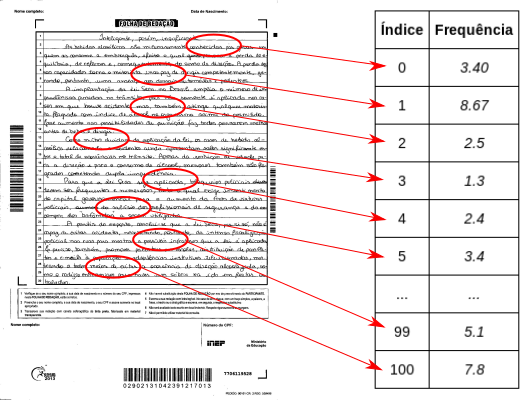
\includegraphics[scale=0.50]{images/bag_of_words.png}
        \end{center}
    \end{figure}

    Matsubara, Martins e Monard (2003) explicam, um dos métodos geralmente 
    adotado para representação estruturada de um texto, é a abordagem 
    bag-of-words \cite{matsubara2003pretext} .

  \end{frame}

  \begin{frame}[fragile]{Naive Bayes}
    \begin{figure}[H]
        \begin{center}
            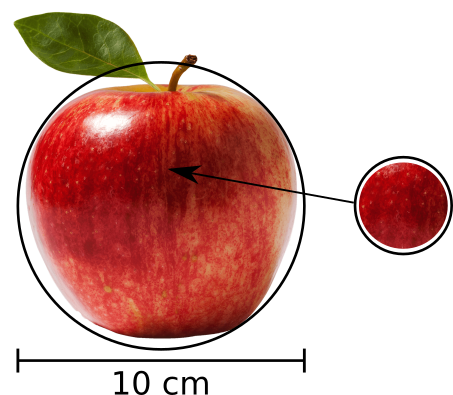
\includegraphics[scale=0.50]{images/naive_bayes.png}
        \end{center}
    \end{figure}
    Brito (2017) descreve em sua pesquisa, o classificador Naive Bayes como 
    um progenitor probabilístico \cite{de2017mineraccao}.
  \end{frame}

  \begin{frame}[fragile]{Adaboost}
    \begin{figure}[H]
        \begin{center}
            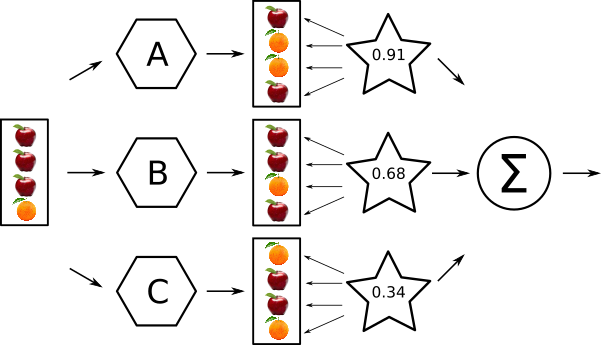
\includegraphics[scale=0.50]{images/adaboost.png}
        \end{center}
    \end{figure}

    Pereira e Ferreira (2015) explicam e sua pesquisa, Adaboost utiliza uma 
    técnica que seleciona diversos algoritmos denominados classificadores 
    fracos, com a finalidade de constituir um classificador forte 
    \cite{pereiraface}.
  \end{frame}

  \begin{frame}[fragile]{Validação cruzada}
    \begin{figure}[H]
        \begin{center}
            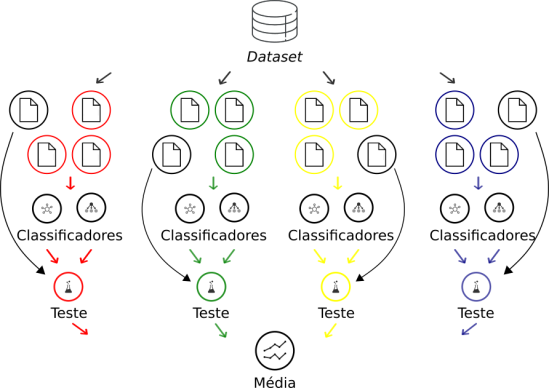
\includegraphics[scale=0.50]{images/validacao_cruzada.png}
        \end{center}
    \end{figure}
    Baker, Isotani e Carvalho (2011) em seu trabalho demonstram, a validação 
    cruzada permite verificar a corretude de um modelo gerado a partir da 
    análise de dados de treinamento \cite{baker2011mineraccao}.
  \end{frame}
